%% ============================================================
%% Quantitative Research -- discussion of Mock Exam 1 (solutions)
%% Layout, colours and code styles as in common/preamble.tex of the lecture.
%% ============================================================
\documentclass[aspectratio=169,11pt]{beamer}

\usepackage[utf8]{inputenc}
\usepackage[T1]{fontenc}
\usepackage[british]{babel}
\usepackage{graphicx}
\usepackage{booktabs}
\usepackage{amsmath,amssymb,amsfonts}
\usepackage{mathtools}
\usepackage{xcolor}
\usepackage{colortbl}
\usepackage{array}
\usepackage{listings}
\usepackage{hyperref}
\hypersetup{pdftitle={Quantitative Research -- Mock Exam 1 -- Slides},
  pdfauthor={Prof. Dr. Christoph Weisser}}

%% sans-serif \mathrm and \mathbf (as in the lecture decks)
\renewcommand{\bfdefault}{bx}
\DeclareMathAlphabet{\mathrm}{T1}{cmss}{m}{n}
\DeclareMathAlphabet{\mathbf}{T1}{cmss}{bx}{n}
\SetMathAlphabet{\mathrm}{bold}{T1}{cmss}{bx}{n}
\SetMathAlphabet{\mathbf}{bold}{T1}{cmss}{bx}{n}
\SetSymbolFont{operators}{bold}{OT1}{cmss}{bx}{n}
\AtBeginDocument{\SetMathAlphabet{\mathrm}{normal}{T1}{cmss}{m}{n}%
                 \SetMathAlphabet{\mathrm}{bold}{T1}{cmss}{bx}{n}}

\definecolor{hsbiblau}{HTML}{3333B2}
\definecolor{hsbiblaudunkel}{HTML}{1C1C6E}
\definecolor{hsbiorange}{HTML}{E69F00}
\definecolor{hsbigrau}{HTML}{9A9A9A}
\definecolor{hsbirot}{HTML}{C0392B}
\definecolor{hsbigruen}{HTML}{2E8B57}

\usetheme{Madrid}
\usecolortheme{default}
\setbeamertemplate{navigation symbols}{}
\setbeamertemplate{blocks}[rounded][shadow=false]
\setbeamerfont{section in head/foot}{size=\tiny}

\setbeamertemplate{headline}{%
  \leavevmode%
  \hbox{%
    \begin{beamercolorbox}[wd=\paperwidth,ht=2.5ex,dp=1.125ex]{section in head/foot}%
      \scriptsize\insertsectionnavigationhorizontal{\paperwidth}{}{\hskip0pt plus1filll}%
    \end{beamercolorbox}%
  }%
}
\newcommand{\footsection}{%
  \setbox0=\hbox{\insertsection}%
  \ifdim\wd0>0pt\ \textbar\ \insertsection\fi}
\setbeamertemplate{footline}{%
  \leavevmode%
  \hbox{%
  \begin{beamercolorbox}[wd=\paperwidth,ht=2.5ex,dp=1.125ex]{author in head/foot}%
    \hspace*{2em}Mock Exam~1\footsection\hfill\insertframenumber{}/\inserttotalframenumber\hspace*{2em}%
  \end{beamercolorbox}%
  }%
}

\AtBeginSection[]{%
  \begin{frame}{Overview}
    \tableofcontents[currentsection,sectionstyle=show/shaded,subsectionstyle=show/show/hide]
  \end{frame}
}

\lstdefinestyle{Pystyle}{
  language=Python,
  basicstyle=\ttfamily\footnotesize,
  keywordstyle=\color{hsbiblau},
  commentstyle=\color{hsbigrau}\itshape,
  stringstyle=\color{teal},
  showstringspaces=false,
  literate={~}{{$\sim$}}1,
  upquote=true,
  columns=fixed, basewidth=0.5em
}
\lstdefinestyle{Pyout}{
  language={},
  basicstyle=\ttfamily\scriptsize,
  keywordstyle={}, commentstyle={}, stringstyle={},
  columns=fixed, keepspaces=true, basewidth=0.52em,
  showstringspaces=false,
  upquote=true
}
\lstset{style=Pystyle}

\renewcommand{\textasciitilde}{\ensuremath{\sim}}
\newcommand{\kernaussage}[1]{\begin{alertblock}{Key takeaway}#1\end{alertblock}}
\newcommand{\inworten}[1]{{\small\textbf{\textcolor{hsbiblaudunkel}{In words:}}~#1}}

\title{Quantitative Research -- Mock Exam 1}
\subtitle{Discussion of the solutions}
\author{Prof.\ Dr.\ Christoph Weisser}
\institute{}
\date{}

\begin{document}

\begin{frame}
  \titlepage
\end{frame}

\begin{frame}{Contents}
  \tableofcontents[hideallsubsections]
\end{frame}

\begin{frame}{The mock exam at a glance}
  \begin{center}\small
  \renewcommand{\arraystretch}{1.2}
  \begin{tabular}{@{}c>{\raggedright\arraybackslash}p{5.6cm}>{\raggedright\arraybackslash}p{4.8cm}c@{}}
    \toprule
    Task & Topic & Scenario & Points\\
    \midrule
    1 & Statistical inference: \texorpdfstring{$z$}{z}-test and confidence interval & Order values of an online shop & 20\\
    2 & Simple and multiple linear regression & Temperature and iced-coffee sales of a caf\'e & 20\\
    3 & Classification: logistic regression and evaluation & Churn prediction of a mobile-phone provider & 20\\
    \midrule
    \multicolumn{3}{@{}l}{\textbf{Total} \hfill 3 $\times$ 10 subtasks worth 2 points each} & \textbf{60}\\
    \bottomrule
  \end{tabular}
  \end{center}
  \medskip
  \begin{block}{How the exam is built}
    Every subtask can be solved \textbf{independently} and asks for exactly \textbf{one} result.
    No intermediate result is needed in a later subtask -- all values required are stated in
    the subtask itself.
  \end{block}
\end{frame}

%====================================================================
\section[Task 1]{Task 1: Statistical inference: \texorpdfstring{$z$}{z}-test and confidence interval}

\begin{frame}{Task 1 -- scenario}
\begin{block}{Order values after the website redesign}
    Planning figure $\mu_0 = 80$~EUR, \quad known $\sigma = 12$~EUR\\[2pt]
    Random sample: $n = 36$ orders, \quad $\bar x = 84.30$~EUR, \quad $\alpha = 0.05$
  \end{block}
  \begin{itemize}\setlength{\itemsep}{3pt}
    \item Question: has the mean order value \emph{changed} (in either direction)?
          $\Rightarrow$ \textbf{two-sided} test.
    \item $\sigma$ known $\Rightarrow$ $Z_n$ and the $\Phi$-table; \ $\sqrt{36} = 6$ keeps the numbers clean.
  \end{itemize}
\end{frame}

\begin{frame}{Task 1 -- the concepts you need}
  \begin{itemize}\setlength{\itemsep}{3pt}
    \item \textbf{Standard error} ($\sigma$ known): $\mathrm{SE} = \sigma/\sqrt{n}$ -- how strongly $\bar X$ fluctuates around $\mu$.
    \item \textbf{Test statistic:} $Z_n = \dfrac{\bar X-\mu_0}{\sigma/\sqrt{n}} \sim N(0,1)$ under $H_0$; two-sided: reject $H_0$ if $|Z_n| > z_{1-\alpha/2}$.
    \item \textbf{$p$-value} (two-sided): $p = 2\,\Phi(-|Z_n|)$; reject $H_0$ if $p < \alpha$.
    \item \textbf{Confidence interval:} $\text{CI}_{1-\alpha} = \bigl[\bar X \pm z_{1-\alpha/2}\,\sigma/\sqrt{n}\bigr]$; $\mu_0$ outside the CI $\Leftrightarrow$ reject $H_0$ (duality).
    \item \textbf{Type~I error:} reject $H_0$ although $H_0$ is true (false alarm); its probability is $\alpha$.
  \end{itemize}
\end{frame}

\begin{frame}{Task 1 -- the test step by step}
  \begin{center}\small
  \renewcommand{\arraystretch}{1.3}
  \begin{tabular}{@{}llll@{}}
    \toprule
    Step & Formula & Numbers & Value\\
    \midrule
    Hypotheses & $H_0\colon\mu = \mu_0$ vs.\ $H_1\colon\mu \neq \mu_0$ & $\mu_0 = 80$ & two-sided\\
    Standard error & $\sigma/\sqrt{n}$ & $12/\sqrt{36}$ & $2$\\
    Test statistic & $Z_n = (\bar x-\mu_0)/(\sigma/\sqrt{n})$ & $(84.30-80)/2$ & $2.15$\\
    Critical value & $z_{1-\alpha/2}$ & $z_{0.975}$ & $1.96$\\
    Decision & $|Z_n| > z_{1-\alpha/2}$\,? & $2.15 > 1.96$ & reject $H_0$\\
    $p$-value & $2\,\Phi(-|Z_n|)$ & $2\,(1-0.9842)$ & $0.0316$\\
    $95\,\%$ CI & $\bar x \pm z_{0.975}\,\sigma/\sqrt{n}$ & $84.30 \pm 3.92$ & $[80.38;\ 88.22]$\\
    \bottomrule
  \end{tabular}
  \end{center}
\end{frame}

\begin{frame}{Task 1 -- three routes, one verdict}
  \begin{columns}[T]
    \column{0.31\textwidth}
    \begin{block}{Critical value}
      $|Z_n| = 2.15$\\ $z_{0.975} = 1.96$\\[2pt]
      $2.15 > 1.96$\\ $\Rightarrow$ \textbf{reject} $H_0$
    \end{block}
    \column{0.31\textwidth}
    \begin{block}{$p$-value}
      $p = 2\,(1-\Phi(2.15))$\\ $\phantom{p} = 0.0316$\\[2pt]
      $0.0316 < 0.05$\\ $\Rightarrow$ \textbf{reject} $H_0$
    \end{block}
    \column{0.31\textwidth}
    \begin{block}{Confidence interval}
      $[80.38;\ 88.22]$\\ $\mu_0 = 80$ outside\\[2pt]
      \phantom{x}\\ $\Rightarrow$ \textbf{reject} $H_0$
    \end{block}
  \end{columns}
  \medskip
  \begin{itemize}\setlength{\itemsep}{2pt}
    \item Type~I error here: ``the mean changed'' although it is still $80$~EUR -- probability $\alpha = 0.05$.
    \item Critical value in Python: \texttt{stats.norm.ppf(0.975)} $= 1.96$ -- pass $1-\alpha/2$, not $\alpha$.
    \item $\sigma$ unknown in practice: \texttt{stats.ttest\_1samp(orders, popmean=80)} (two-sided by default, $t_{35}$).
  \end{itemize}
  \kernaussage{Critical value, $p$-value and CI are three views of the same test -- they always agree.}
\end{frame}

\begin{frame}{Task 1 -- results a)--e)}
  \begin{center}\small
  \renewcommand{\arraystretch}{1.35}
  \begin{tabular}{@{}c>{\raggedright\arraybackslash}p{4.9cm}>{\raggedright\arraybackslash}p{8.4cm}@{}}
    \toprule Part & Asked for & Result\\ \midrule
    \textbf{a)} & Hypothesis pair & $H_0\colon \mu = 80$ vs.\ $H_1\colon \mu \neq 80$\\
    \textbf{b)} & Standard error & $\sigma/\sqrt{n} = 12/6 = 2$~EUR\\
    \textbf{c)} & Test statistic $Z_n$ & $Z_n = 4.30/2 = 2.15$\\
    \textbf{d)} & Python: critical value with \texttt{stats.norm.ppf} & \texttt{q} $= 1-\alpha/2 = 0.975$ \ (returns $z_{0.975} = 1.96$)\\
    \textbf{e)} & Test decision & $|Z_n| = 2.15 > 1.96$ $\Rightarrow$ reject $H_0$\\
    \bottomrule
  \end{tabular}
  \end{center}
\end{frame}

\begin{frame}{Task 1 -- results f)--j)}
  \begin{center}\small
  \renewcommand{\arraystretch}{1.35}
  \begin{tabular}{@{}c>{\raggedright\arraybackslash}p{4.9cm}>{\raggedright\arraybackslash}p{8.4cm}@{}}
    \toprule Part & Asked for & Result\\ \midrule
    \textbf{f)} & $p$-value & $p = 2\,(1-0.9842) = 0.0316$\\
    \textbf{g)} & $95\,\%$ confidence interval & $84.30 \pm 3.92 = [80.38;\ 88.22]$~EUR\\
    \textbf{h)} & Interpretation of the CI & with $95\,\%$ confidence, the mean $\mu$ of \emph{all} orders lies in $[80.38;\ 88.22]$~EUR\\
    \textbf{i)} & Type I error in context & rejecting $H_0$ (``mean changed'') although $\mu = 80$~EUR still holds\\
    \textbf{j)} & Python command ($t$-test) & \texttt{stats.ttest\_1samp(orders, popmean=80)}\\
    \bottomrule
  \end{tabular}
  \end{center}
\end{frame}

\begin{frame}{Task 1 -- rejection region and test statistic}
  \begin{center}
    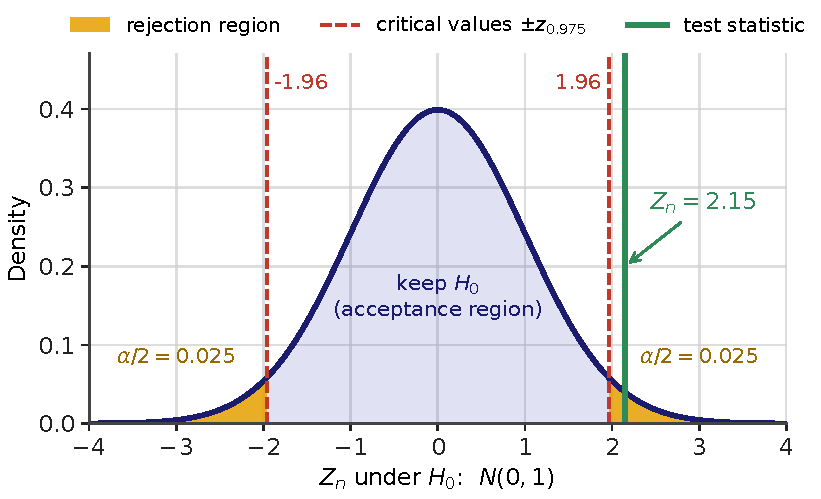
\includegraphics[width=\textwidth,height=0.78\textheight,keepaspectratio]{qrm1_t1_ztest.pdf}
  \end{center}
\end{frame}

\begin{frame}{Task 1 -- confidence interval and duality}
  \begin{center}
    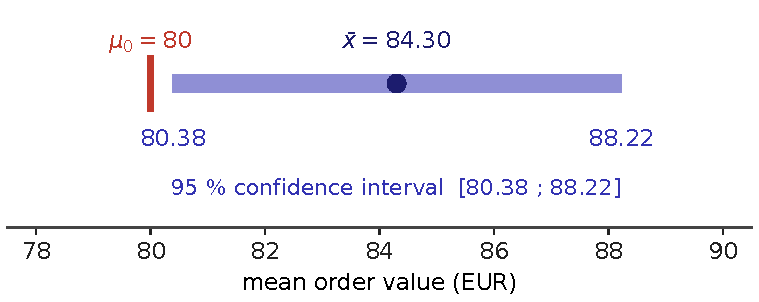
\includegraphics[width=\textwidth,height=0.62\textheight,keepaspectratio]{qrm1_t1_ci.pdf}
  \end{center}
\end{frame}

\begin{frame}{Task 1 -- typical mistakes}
  \begin{itemize}\setlength{\itemsep}{4pt}
    \item Using the one-sided quantile $z_{0.95} = 1.645$ for the two-sided test -- in Python \texttt{stats.norm.ppf(0.95)} instead of \texttt{stats.norm.ppf(0.975)}.
    \item Forgetting the factor $2$ in the two-sided $p$-value ($0.0158$ instead of $0.0316$).
    \item Standard error with $n$ or $n-1$ instead of $\sqrt{n}$.
    \item Reading the CI as the range of single order values, or as ``$95\,\%$ probability for \emph{this} interval''.
    \item Mixing up the Type~I error (false alarm: reject a true $H_0$) and the Type~II error (miss).
  \end{itemize}
\end{frame}


%====================================================================
\section[Task 2]{Task 2: Simple and multiple linear regression}

\begin{frame}{Task 2 -- scenario}
\begin{columns}[T]
    \column{0.47\textwidth}
    \begin{block}{Part A: five summer days}
      \begin{center}\small
      \begin{tabular}{lccccc}
        \toprule
        $x_i$ ($^{\circ}$C) & 20 & 22 & 24 & 26 & 28\\
        $y_i$ & 46 & 54 & 62 & 70 & 68\\
        \bottomrule
      \end{tabular}
      \end{center}
      \small $\bar x = 24$, $\bar y = 60$\\
      $S_{xx} = 40$, $S_{xy} = 120$, $S_{yy} = 400$
    \end{block}
    \column{0.49\textwidth}
    \begin{block}{Part B: 60 days, two explanatory variables}
      \small \texttt{sales \textasciitilde{} temp + rain}\\[3pt]
      \begin{tabular}{lrr}
        \toprule
        & coef & \texttt{P>|t|}\\
        \midrule
        \texttt{temp} & $3.0055$ & $0.000$\\
        \texttt{rain} & $-0.4313$ & $0.253$\\
        \bottomrule
      \end{tabular}
    \end{block}
  \end{columns}
\end{frame}

\begin{frame}{Task 2 -- the concepts you need}
  \begin{itemize}\setlength{\itemsep}{3pt}
    \item \textbf{OLS estimators:} $\hat\beta_1 = S_{xy}/S_{xx}$, \ $\hat\beta_0 = \bar y - \hat\beta_1\bar x$; \ line $\hat y = \hat\beta_0 + \hat\beta_1 x$.
    \item \textbf{Residual:} $\hat u_i = y_i - \hat y_i$ -- positive: point above the line, negative: below.
    \item \textbf{Sum-of-squares decomposition:} $\text{TSS} = \text{ESS} + \text{RSS}$, \ $R^2 = \text{ESS}/\text{TSS} = 1 - \text{RSS}/\text{TSS}$.
    \item \textbf{Correlation} (simple regression): $R^2 = r_{xy}^2$, so $r_{xy} = \pm\sqrt{R^2}$ with the sign of $\hat\beta_1$.
    \item \textbf{Multiple regression:} $\hat\beta_j$ = change of $y$ per unit of $x_j$ \emph{holding the other variables fixed}; $H_0\colon \beta_j = 0$ is rejected if $p < \alpha$.
  \end{itemize}
\end{frame}

\begin{frame}{Task 2 -- line, fitted values and residuals}
  \[ \hat\beta_1 = \frac{S_{xy}}{S_{xx}} = \frac{120}{40} = 3, \qquad
     \hat\beta_0 = \bar y - \hat\beta_1\bar x = 60 - 3\cdot 24 = -12
     \qquad\Rightarrow\qquad \hat y = -12 + 3x \]
  \begin{center}\small
  \renewcommand{\arraystretch}{1.2}
  \begin{tabular}{lccccc|c}
    \toprule
    $x_i$ & 20 & 22 & 24 & 26 & 28 & $\sum$\\
    $y_i$ & 46 & 54 & 62 & 70 & 68 & 300\\
    $\hat y_i$ & 48 & 54 & 60 & 66 & 72 & 300\\
    $\hat u_i = y_i - \hat y_i$ & $-2$ & $0$ & $+2$ & $+4$ & $-4$ & $0$\\
    $\hat u_i^{\,2}$ & 4 & 0 & 4 & 16 & 16 & $40 = \text{RSS}$\\
    \bottomrule
  \end{tabular}
  \end{center}
  \begin{itemize}\setlength{\itemsep}{2pt}
    \item Prediction at $x = 25$ (inside the data range): $\hat y = -12 + 75 = 63$ -- in Python \texttt{reg.predict(pd.DataFrame(\{"temp":\ [25]\}))}.
    \item Slope: $1$\,$^{\circ}$C warmer $\Rightarrow$ on average $3$ more iced coffees; the intercept $-12$ is pure extrapolation.
  \end{itemize}
\end{frame}

\begin{frame}{Task 2 -- sums of squares, $R^2$ and $r_{xy}$}
  \[ \underbrace{\text{TSS}}_{S_{yy} = 400} \;=\; \underbrace{\text{ESS}}_{\hat\beta_1^2 S_{xx} = 9\cdot 40 = 360}
     \;+\; \underbrace{\text{RSS}}_{\sum\hat u_i^2 = 40} \]
  \[ R^2 = \frac{\text{ESS}}{\text{TSS}} = 1 - \frac{\text{RSS}}{\text{TSS}} = 1 - \frac{40}{400} = 0.9,
     \qquad r_{xy} = +\sqrt{0.9} = 0.9487 \]
  \begin{itemize}\setlength{\itemsep}{3pt}
    \item $90\,\%$ of the variation in sales is explained (linearly) by the temperature.
    \item The sign of $r_{xy}$ comes from $\hat\beta_1 > 0$; check: $120/\sqrt{40\cdot 400} = 0.9487$.
  \end{itemize}
  \kernaussage{$R^2 = r_{xy}^2$ holds in \emph{simple} regression only -- take the root and add the sign of the slope.}
\end{frame}

\begin{frame}[fragile]{Task 2 -- reading the multiple regression output}
\begin{lstlisting}[style=Pyout]
Dep. Variable:                  sales   R-squared:                       0.947
Model:                            OLS   Adj. R-squared:                  0.945
Method:                 Least Squares   F-statistic:                     512.4
                 coef    std err          t      P>|t|      [0.025      0.975]
------------------------------------------------------------------------------
Intercept    -12.2152      3.783     -3.229      0.002     -19.790      -4.641
temp           3.0055      0.131     22.863      0.000       2.742       3.269
rain          -0.4313      0.374     -1.154      0.253      -1.180       0.317
\end{lstlisting}
  \begin{itemize}\setlength{\itemsep}{2pt}\small
    \item \texttt{temp}: holding \texttt{rain} fixed, $+1$\,$^{\circ}$C $\Rightarrow$ on average $+3.01$ iced coffees ($p = 0.000$).
    \item \texttt{rain}: $p = 0.253 > 0.05$ $\Rightarrow$ keep $H_0\colon \beta_2 = 0$ -- not significant \emph{given the temperature}.
    \item Confounding: alone, \texttt{sales \textasciitilde{} rain} has slope $-6.19$ -- rainy days are also cooler days.
  \end{itemize}
\end{frame}

\begin{frame}{Task 2 -- results a)--e)}
  \begin{center}\small
  \renewcommand{\arraystretch}{1.35}
  \begin{tabular}{@{}c>{\raggedright\arraybackslash}p{4.9cm}>{\raggedright\arraybackslash}p{8.4cm}@{}}
    \toprule Part & Asked for & Result\\ \midrule
    \textbf{a)} & Slope $\hat\beta_1$ & $\hat\beta_1 = 120/40 = 3$\\
    \textbf{b)} & Intercept $\hat\beta_0$ & $\hat\beta_0 = 60 - 3\cdot 24 = -12$\\
    \textbf{c)} & Interpretation of the slope & $1$\,$^{\circ}$C warmer $\Rightarrow$ on average about $3$ more iced coffees sold\\
    \textbf{d)} & Python: prediction with \texttt{reg.predict} & $\hat y(25) = -12 + 3\cdot 25 = 63$ iced coffees\\
    \textbf{e)} & Residual of day 5 & $\hat u_5 = 68 - 72 = -4$\\
    \bottomrule
  \end{tabular}
  \end{center}
\end{frame}

\begin{frame}{Task 2 -- results f)--j)}
  \begin{center}\small
  \renewcommand{\arraystretch}{1.35}
  \begin{tabular}{@{}c>{\raggedright\arraybackslash}p{4.9cm}>{\raggedright\arraybackslash}p{8.4cm}@{}}
    \toprule Part & Asked for & Result\\ \midrule
    \textbf{f)} & Coefficient of determination $R^2$ & $R^2 = 1 - 40/400 = 0.9$\\
    \textbf{g)} & Correlation coefficient $r_{xy}$ & $r_{xy} = +\sqrt{0.9} = 0.9487$\\
    \textbf{h)} & Python command (OLS) & \texttt{smf.ols("sales \textasciitilde{} temp", data=cafe).fit()}\\
    \textbf{i)} & Ceteris-paribus interpretation & holding rain fixed: $+1$\,$^{\circ}$C $\Rightarrow$ on average $3.01$ more iced coffees\\
    \textbf{j)} & Significance of \texttt{rain} & $p = 0.253 > 0.05$ $\Rightarrow$ not significant (keep $H_0\colon \beta_2 = 0$)\\
    \bottomrule
  \end{tabular}
  \end{center}
\end{frame}

\begin{frame}{Task 2 -- scatter plot, OLS line and residuals}
  \begin{center}
    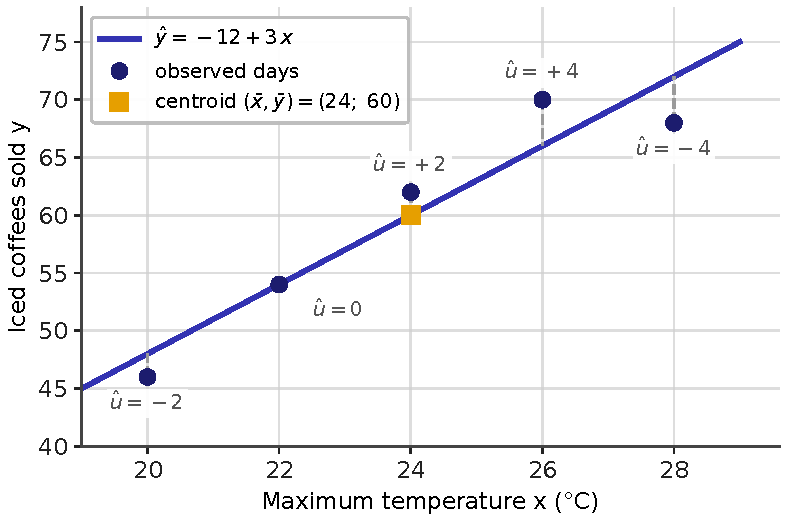
\includegraphics[width=\textwidth,height=0.78\textheight,keepaspectratio]{qrm1_t2_scatter.pdf}
  \end{center}
\end{frame}

\begin{frame}{Task 2 -- typical mistakes}
  \begin{itemize}\setlength{\itemsep}{4pt}
    \item $\hat\beta_1 = S_{xx}/S_{xy}$ instead of $S_{xy}/S_{xx}$.
    \item Residual with the wrong sign ($\hat y_i - y_i$ instead of $y_i - \hat y_i$).
    \item $r_{xy} = R^2$, or the sign of $r_{xy}$ ignored.
    \item Slope interpreted without units or as a proven causal effect.
    \item Multiple regression: the clause ``holding the other variables fixed'' forgotten; ``not significant'' read as ``no effect''.
  \end{itemize}
\end{frame}


%====================================================================
\section[Task 3]{Task 3: Classification: logistic regression and evaluation}

\begin{frame}{Task 3 -- scenario}
\begin{columns}[T]
    \column{0.50\textwidth}
    \begin{block}{Logistic regression}
      $Y = 1$: customer cancels (churn)\\
      $x$: hotline calls in the last six months\\[4pt]
      $\hat\eta(x) = -3 + 0.5\,x$\\[3pt]
      $\hat p(x) = \dfrac{e^{\hat\eta}}{1+e^{\hat\eta}}$
    \end{block}
    \column{0.46\textwidth}
    \begin{block}{Test data, $t = 0.5$}
      \begin{center}\small
      \begin{tabular}{l|cc|c}
        & Pred.\ No & Pred.\ Yes & \\
        \hline
        Act.\ No & 140 & 20 & 160\\
        Act.\ Yes & 10 & 30 & 40\\
        \hline
        & 150 & 50 & 200
      \end{tabular}
      \end{center}
    \end{block}
  \end{columns}
\end{frame}

\begin{frame}{Task 3 -- the concepts you need}
  \begin{itemize}\setlength{\itemsep}{3pt}
    \item \textbf{Odds:} $\text{odds} = \dfrac{p}{1-p}$; back: $p = \dfrac{\text{odds}}{1+\text{odds}}$.
    \item \textbf{Logistic model:} linear predictor $\eta = \beta_0 + \beta_1 x$ (log-odds), \ $p(x) = \dfrac{e^{\eta}}{1+e^{\eta}}$.
    \item \textbf{Odds ratio} $e^{\beta_1}$: factor by which the \emph{odds} change per additional unit of $x$.
    \item \textbf{Classification rule:} $\hat y = 1$ if $\hat p(x) > t$; \ $t = 0.5 \Leftrightarrow \hat\eta(x) > 0$.
    \item \textbf{Confusion matrix:} accuracy $= (\mathrm{TP}+\mathrm{TN})/n$, sensitivity $= \mathrm{TP}/(\mathrm{TP}+\mathrm{FN})$, specificity $= \mathrm{TN}/(\mathrm{TN}+\mathrm{FP})$, precision $= \mathrm{TP}/(\mathrm{TP}+\mathrm{FP})$.
  \end{itemize}
\end{frame}

\begin{frame}{Task 3 -- from hotline calls to a decision}
  \begin{center}\small
  \renewcommand{\arraystretch}{1.25}
  \begin{tabular}{cccccc}
    \toprule
    calls $x$ & $\hat\eta = -3 + 0.5x$ & odds $= e^{\hat\eta}$ & $\hat p = \frac{\text{odds}}{1+\text{odds}}$ & $\hat y$ ($t = 0.5$) & $\hat y$ ($t = 0.3$)\\
    \midrule
    2 & $-2.0$ & $0.1353$ & $0.1192$ & 0 & 0\\
    4 & $-1.0$ & $0.3679$ & $0.2689$ & 0 & 0\\
    5 & $-0.5$ & $0.6065$ & $0.3775$ & 0 & \textbf{1}\\
    6 & $\phantom{-}0.0$ & $1.0000$ & $0.5000$ & 0 & \textbf{1}\\
    7 & $\phantom{-}0.5$ & $1.6487$ & $0.6225$ & \textbf{1} & \textbf{1}\\
    \bottomrule
  \end{tabular}
  \end{center}
  \begin{itemize}\setlength{\itemsep}{2pt}
    \item Odds of churn overall: $0.2/0.8 = 0.25$.
    \item One call more: odds $\times\, e^{0.5} = 1.6487$ -- the \emph{odds} rise by $65\,\%$, not the probability.
    \item $t = 0.5 \Leftrightarrow \hat\eta > 0 \Leftrightarrow x \ge 7$; \quad $t = 0.3 \Leftrightarrow \hat\eta > -0.847 \Leftrightarrow x \ge 5$.
  \end{itemize}
\end{frame}

\begin{frame}{Task 3 -- the confusion matrix and its four measures}
  \begin{columns}[c]
    \column{0.42\textwidth}
    \begin{center}\small
    \renewcommand{\arraystretch}{1.3}
    \begin{tabular}{l|cc|c}
      & Pred.\ No & Pred.\ Yes & \\
      \hline
      Act.\ No & \cellcolor{hsbigruen!18}TN $= 140$ & \cellcolor{hsbirot!15}FP $= 20$ & 160\\
      Act.\ Yes & \cellcolor{hsbirot!15}FN $= 10$ & \cellcolor{hsbigruen!18}TP $= 30$ & 40\\
      \hline
      & 150 & 50 & 200
    \end{tabular}
    \end{center}
    \column{0.54\textwidth}
    \begin{block}{Measures (which total do we divide by?)}
      \renewcommand{\arraystretch}{1.3}
      \begin{tabular}{@{}lll@{}}
        Accuracy & $(30+140)/200$ & $= 0.85$\\
        Sensitivity & $30/40$ \ (row Act.\ Yes) & $= 0.75$\\
        Specificity & $140/160$ \ (row Act.\ No) & $= 0.875$\\
        Precision & $30/50$ \ (column Pred.\ Yes) & $= 0.6$
      \end{tabular}
    \end{block}
  \end{columns}
  \medskip
  \kernaussage{Lower threshold $\Rightarrow$ more customers flagged $\Rightarrow$ sensitivity $\uparrow$, specificity $\downarrow$.}
\end{frame}

\begin{frame}{Task 3 -- results a)--e)}
  \begin{center}\small
  \renewcommand{\arraystretch}{1.35}
  \begin{tabular}{@{}c>{\raggedright\arraybackslash}p{4.9cm}>{\raggedright\arraybackslash}p{8.4cm}@{}}
    \toprule Part & Asked for & Result\\ \midrule
    \textbf{a)} & Odds of churn & odds $= 0.2/0.8 = 0.25$\\
    \textbf{b)} & Churn probability at $x = 2$ & $\hat\eta = -2$, \ $\hat p = 0.1353/1.1353 = 0.1192$\\
    \textbf{c)} & Interpretation of the odds ratio & each extra call multiplies the \emph{odds} of churn by $1.65$ ($+65\,\%$)\\
    \textbf{d)} & Classification at $x = 7$ & $\hat\eta = 0.5 > 0$, $\hat p = 0.6225 > 0.5$ $\Rightarrow$ $\hat y = 1$ (churn)\\
    \textbf{e)} & Python command (logit) & \texttt{smf.logit("churn \textasciitilde{} calls", data=df).fit()}\\
    \bottomrule
  \end{tabular}
  \end{center}
\end{frame}

\begin{frame}{Task 3 -- results f)--j)}
  \begin{center}\small
  \renewcommand{\arraystretch}{1.35}
  \begin{tabular}{@{}c>{\raggedright\arraybackslash}p{4.9cm}>{\raggedright\arraybackslash}p{8.4cm}@{}}
    \toprule Part & Asked for & Result\\ \midrule
    \textbf{f)} & Accuracy & $(30 + 140)/200 = 0.85$\\
    \textbf{g)} & Python: row shares with \texttt{pd.crosstab} & row share $30/(30 + 10) = 0.75$ (the sensitivity)\\
    \textbf{h)} & Specificity & $140/(140 + 20) = 0.875$\\
    \textbf{i)} & Precision & $30/(30 + 20) = 0.6$\\
    \textbf{j)} & Lower threshold $t = 0.3$ & sensitivity \textbf{increases} (more churners caught)\\
    \bottomrule
  \end{tabular}
  \end{center}
\end{frame}

\begin{frame}{Task 3 -- the S-curve and the two thresholds}
  \begin{center}
    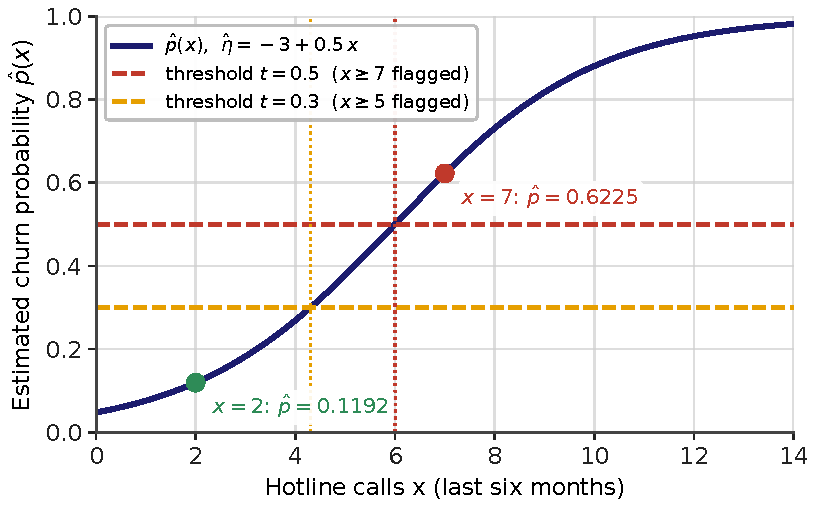
\includegraphics[width=\textwidth,height=0.78\textheight,keepaspectratio]{qrm1_t3_logistic.pdf}
  \end{center}
\end{frame}

\begin{frame}{Task 3 -- typical mistakes}
  \begin{itemize}\setlength{\itemsep}{4pt}
    \item Reading the log-odds $\hat\eta$ (or the odds $e^{\hat\eta}$) as a probability.
    \item ``The odds ratio is $1.65$, so the \emph{probability} rises by $65\,\%$.''
    \item Mixing up sensitivity (divide by \emph{actual} Yes, \texttt{normalize="index"}) and precision (divide by \emph{predicted} Yes, \texttt{normalize="columns"}).
    \item Rows and columns of the confusion matrix confused (specificity $\neq$ $\mathrm{TN}/(\mathrm{TN}+\mathrm{FN})$).
    \item Believing that a lower threshold catches \emph{fewer} churners.
  \end{itemize}
\end{frame}


\section*{Wrap-up}
\begin{frame}{Points and exam strategy}
  \begin{block}{Structure}
    3~tasks $\times$ 10~subtasks $\times$ 2~points = 60~points in 120~minutes
    -- about 4~minutes per subtask.
  \end{block}
  \begin{itemize}\setlength{\itemsep}{4pt}
    \item All subtasks are \textbf{independent}: skip whatever is stuck and come back to it at
      the end -- you lose no further points.
    \item Each subtask asks for \textbf{one} result -- mark it clearly on your working pages.
    \item Still write down your working: a result without working earns only half the points.
    \item Do not forget units, signs and rounding.
  \end{itemize}
\end{frame}

\end{document}
